\chapter{Methods}
\noindent
\section{Computational Methods}
\label{sec:compmeth}

\subsection{Model}
\label{sec:model}
The simulation model consists of a soil block with uniform properties to replicate real-world conditions as much as possible but also to the extent that the model can allow. Steel was chosen as the material for the rod to be used with a hydraulic jack of 1000KN to ensure effective load transmission to the pipe.

The model is built using COMSOL Multiphysics using the solid mechanic model to simulate the effect of load on the pipe. The enhanced model was imported into Matlab, where random values were assigned to the pipe and load properties to simulate various scenarios. This step was essential for generating a comprehensive dataset.

\begin{figure}[t]
    \centering
    \begin{subfigure}[b]{0.4\textwidth}
        \centering
        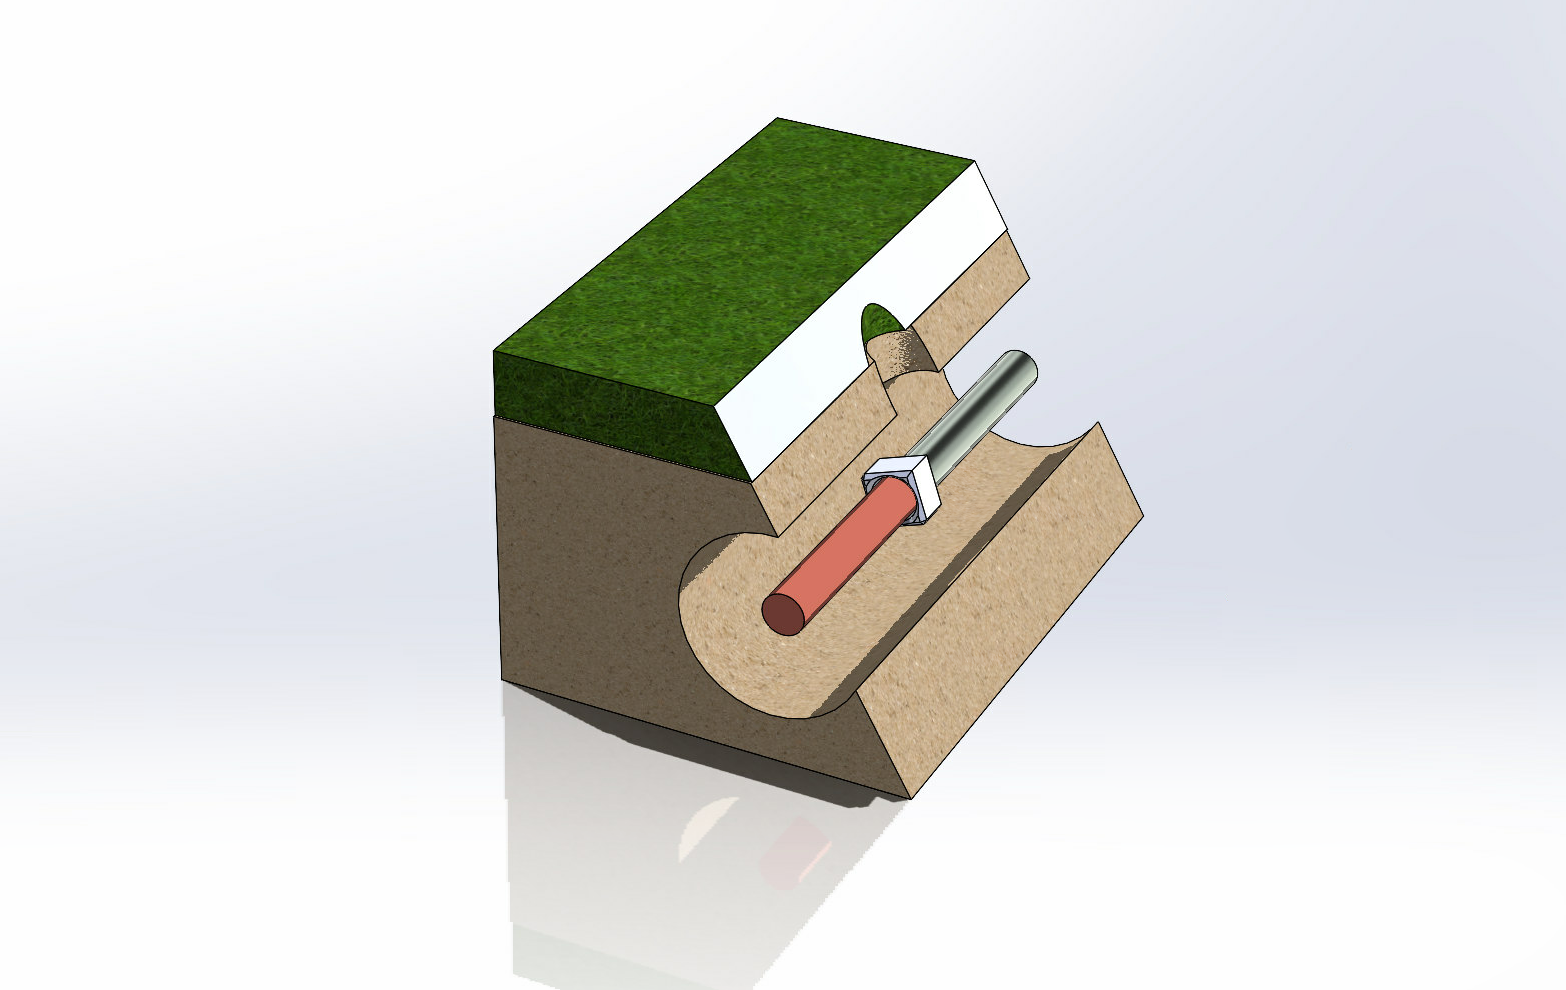
\includegraphics[width=\textwidth]{./Section_2.png}
        \caption{Section of the buried Copper and Lead Pipe}
        \label{fig:sub1}
    \end{subfigure}
    \hfill
    \begin{subfigure}[b]{0.4\textwidth}
        \centering

        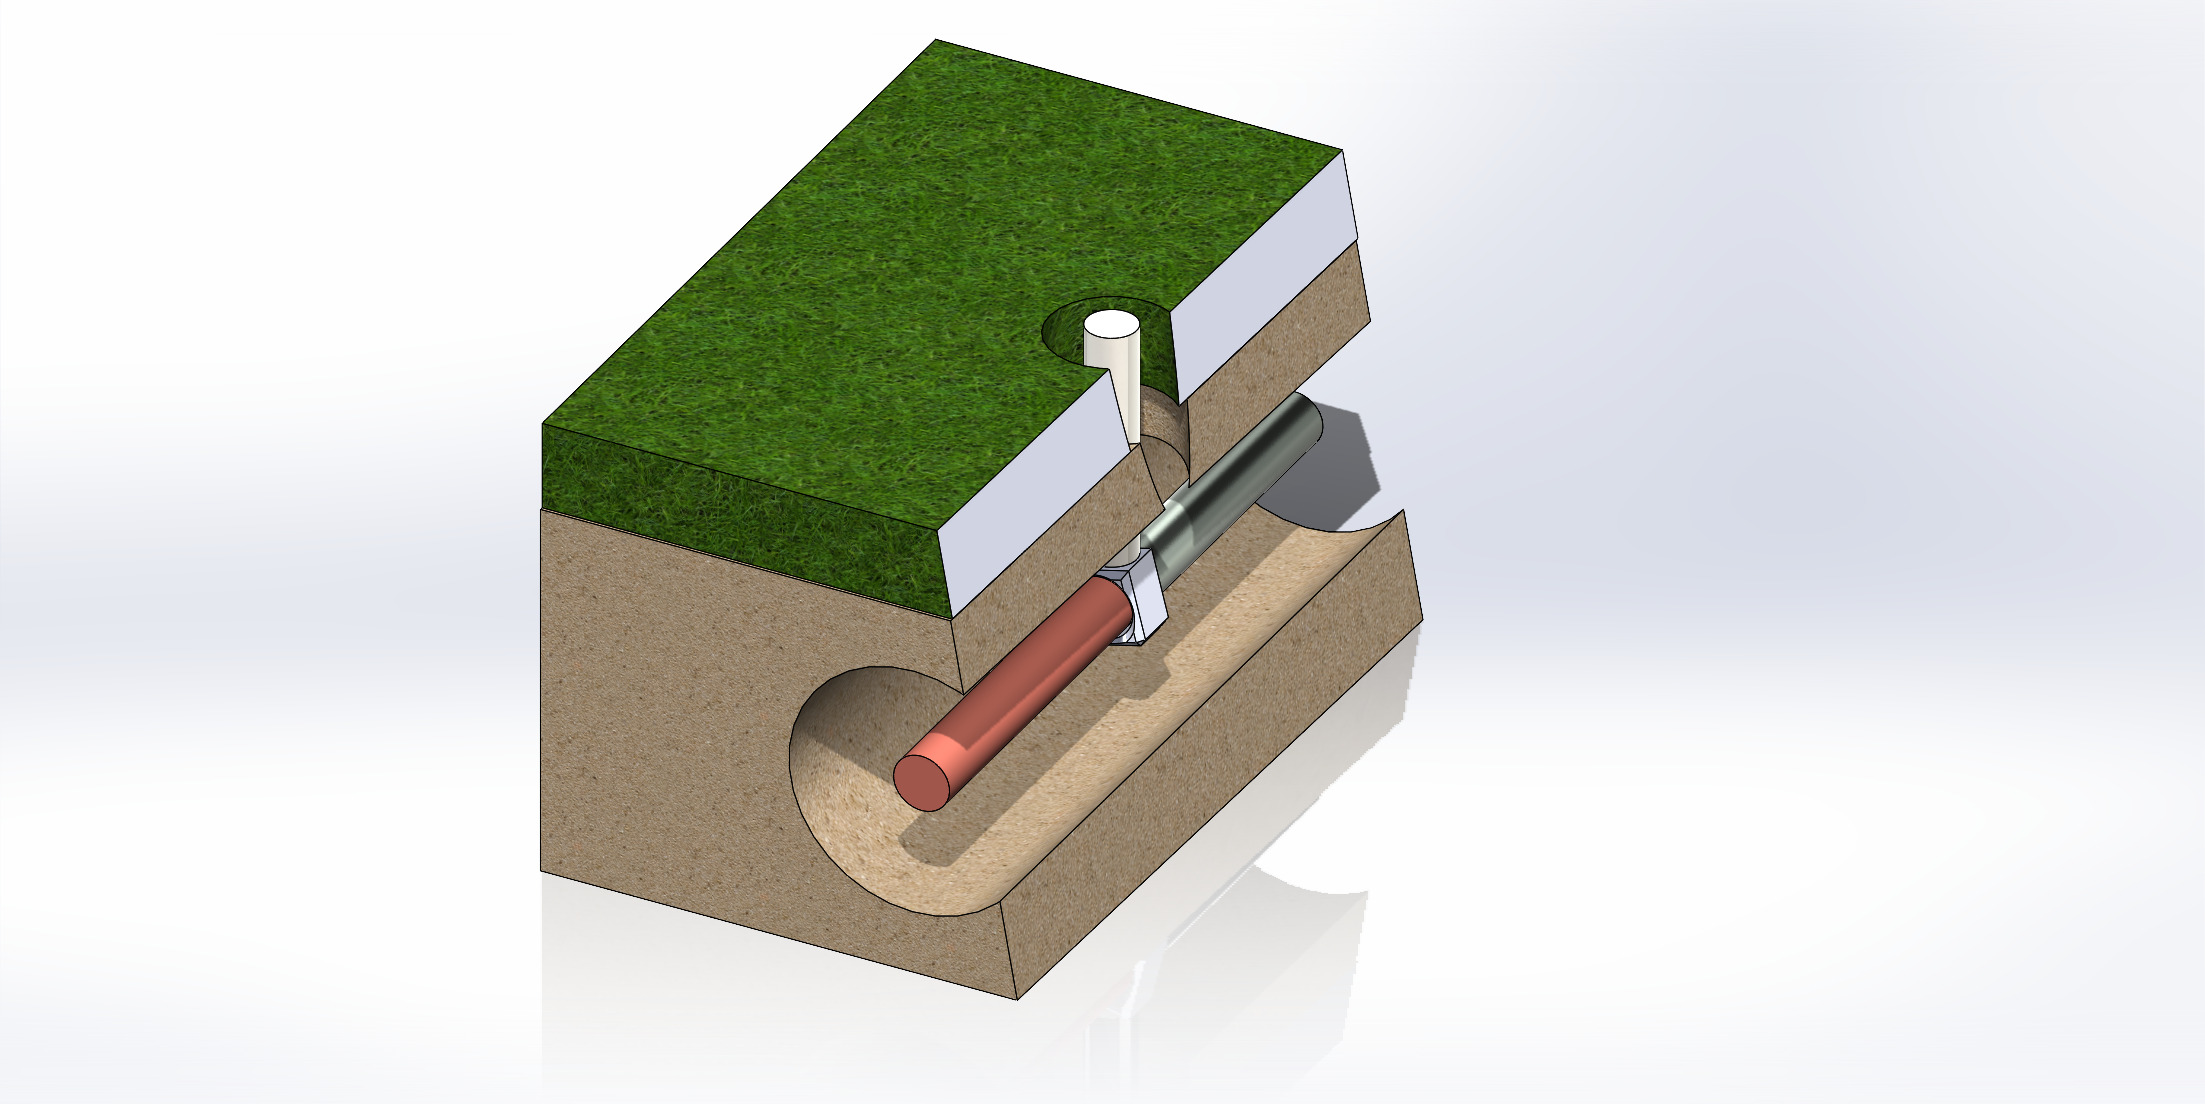
\includegraphics[width=\textwidth]{./Complete.jpg}
        \caption{Section of the buried Copper and Lead Pipe with steel rod}
        \label{fig:sub2}
    \end{subfigure}
    \caption{Section of the buried Copper and Lead Pipe with steel rod}
    \label{fig:main}
\end{figure}



\subsection{Dataset Generation}
Approximately 5000 datasets were generated to train the machine learning model. The large dataset is critical for improving the accuracy and reliability of the CNN used for detection.

\begin{figure}[t]
    \centering
    \begin{subfigure}[b]{0.4\textwidth}
        \centering
        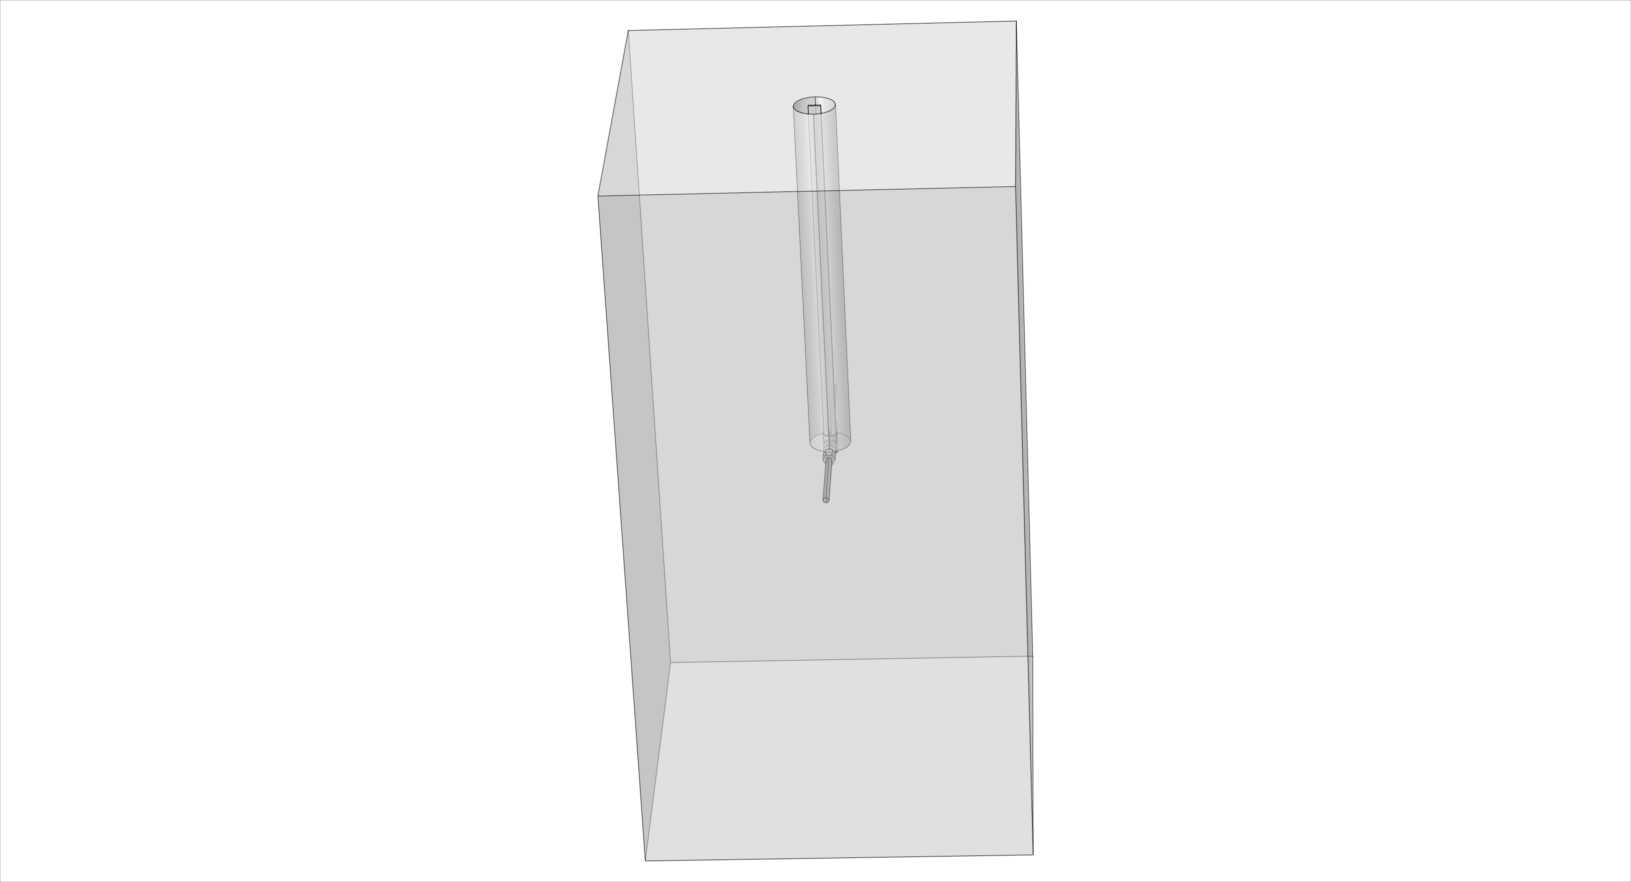
\includegraphics[width=\textwidth]{./Model_Image.png}
        \caption{Side View}
        \label{fig:sub1}
    \end{subfigure}
    \hfill
    \begin{subfigure}[b]{0.4\textwidth}
        \centering
        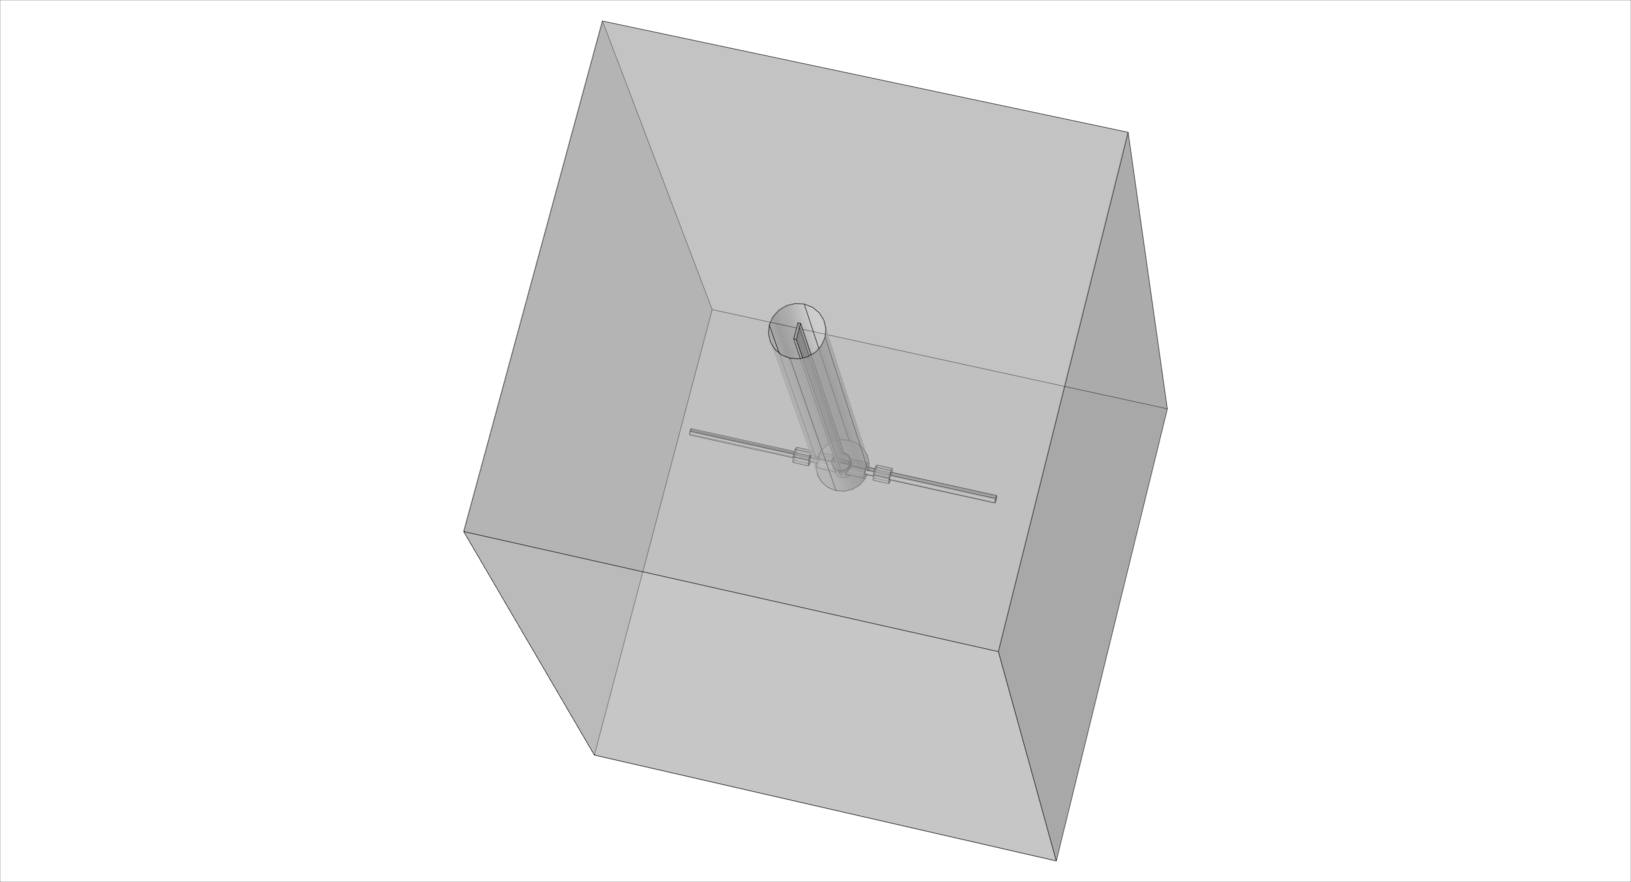
\includegraphics[width=\textwidth]{./Model_Image_12.png}
        \caption{Top View}
        \label{fig:sub2}
    \end{subfigure}
    \caption{Side and Top View of the Solid}
    \label{fig:main}
\end{figure}


\begin{equation}
  \rho \left( \frac{\partial^2 u}{\partial t^2} \right) = \nabla \cdot \mathbf{S} + \mathbf{F}_v
\end{equation}


\subsubsection{Data Categorization}
The generated data was separated into two categories: lead and copper. This categorization enabled the CNN to learn the distinct characteristics of each metal.

\subsubsection{Model Training}
The categorized data was used to train the CNN, aiming to develop a robust detection system capable of identifying the presence of lead and copper pipes that are buried withiout digging, thus saving cost.

 

% Uncomment for bibliography on each chapter.
% \bibliographystyle{plainnat}				
% \markright{\textit{Bibliography}}
% \renewcommand{\chaptername}{}
% \bibliography{my_references}

% \vfill


%%% Local Variables:
%%% mode: latex
%%% TeX-master: "DMSE-Thesis"
%%% End:
